\chapter{Methods}

\subsection{Frequency-Domain Learning}
% TODO: related rationale in Minimum-variance by f. gran and jorgen jensen in frequency domain.

Even though it would be intuitive to simply denoise our raw channel data (in the time domain) along the aperture because off-axis scattering and reverberation are defined across the channel, time-domain ultrasound signals are subject to the issue of depth-dependent attenuation, which describes the loss of acoustic energy as the signal travels through a medium. Depth-dependent attenuation is not only a function of time/distance, but also of frequency. If we train on time signal, it is possible that we will need to learn this function in addition to denoising. Our hypothesis is that because depth-dependent attenuation is a function of both time and frequency, it would be intractible to learn given only time-domain data. Therefore, we can circumvent this issue by using processing the signal amplitude across the channel per frequency. Because the 4th, 5th, and 6th frequencies are most affected, we can save our efforts by only training one model for each of these three frequencies.

In order to extract the frequency-domain data from time-domain channel data, we use the short-time Fourier transform (STFT) on the time-domain channel data to generate a time-frequency spectrogram that we call STFT-domain data. The original time dimension is consumed to produce the frequency dimension and the time segments dimension. As a result, the data dimensionality increases to 4D: the number of frequencies, the number of segments, the number of channels per beam, and the number of beams. The value of each data point changes from voltage to complex amplitude data consisting of the real in-phase (I) and the imaginary quadrature (Q) componenets.

Additional benefits to training in the STFT domain include resilience to changes in pulse shape which only affects the time domain. Lastly, being able to use complex data instead of relying on the Hilbert transform is another benefit of training in the STFT domain.


\begin{figure}
  \centerline{\includegraphics[width=6.5in,scale=0.7]{training_data_modes.png}}
  \caption{The simulated training data has three modes: accept, reject, and discriminate.}
  \label{fig:training_data_modes}
\end{figure}

The learning task is preserving the signal component of frequency-domain input data while discarding (zeroing out) the noise component. More specifically, there are three cases of input signals: accept, reject, and mixed. If a frequency-domain input signal falls inside the main lobe of a beam (accept case), the target signal to learn is the same as the input. In other words, the mapping from inputs to targets in the accept case is the identity function. In ther reject case, the targets are set to 0s as they are all frmo the off-axis region. In the mixed case, however, there are signals from both inside and outside the main lobe. The targets, in this case, is the inside component of the mixed signal, which is accessible from the simulation. The learning task here is to discriminate between the signal and the noise and only preserve the signal component. Figure \ref{fig:training_data_modes} shows these three modes.


\section{Training Data Generation}

The training dataset in this thesis was generated by Luchies and Byram for their MLP denoising studies \cite{luchies_tmi_2018}. Training data was generated from Field II \cite{jensen1992calculation, jensen1996field} simulated point target responses. The simulated ultrasonic array was based on the L7-4 (38 mm) linear array transducer. Point targets were randomly placed in an annular sector centered at the focal depth of the transducer array \cite{training_improvements}. Both inputs and targets have been delayed and have gone through the STFT step. The number of elements per beam is 65. We used $10^5$ examples for training and $10^4$ for validation.
% TODO: verify the mixed case target generation process.

% TODO: Ask Brett again on how to explain why smoothing.



% TODO: annular scatterer plot by Adam. Figure 3 Scatterers were randomly placed along the annular sector as depicted. The acceptance region was taken as the region between the first nulls of a simulated beam. Question: Cite this figure? Not mine.



% TODO: Should I talk about convolution at all? Probably should because 1. I talk about 1D vs 2D convolution. 2. I talk about CNR as a function of increasing kernel size and what that implies.
% TODO: Talk about receptive field for convolution

% \section{Convolution}



% TODO: Should I put groupings in this at all?
\section{Grouping of Real and Imaginary Input Componenets}
\begin{figure}
  \centerline{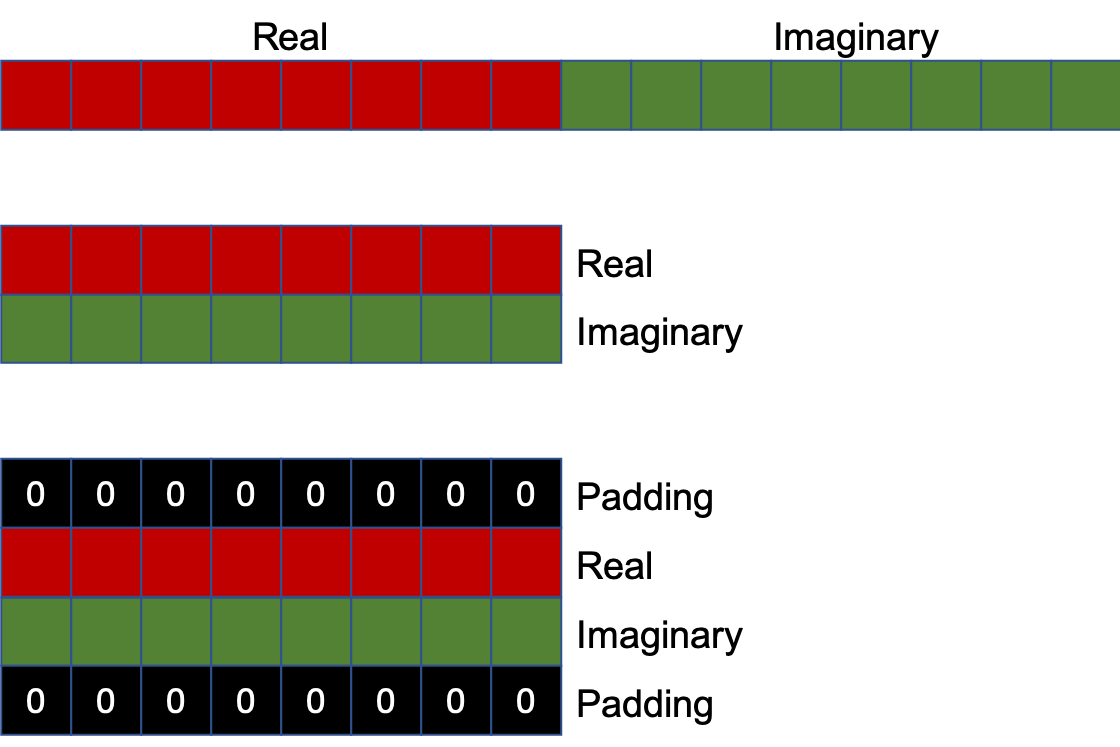
\includegraphics[width=85mm,scale=0.5]{iq_groupings.png}}
  \caption{Top to bottom: 1D, single-channel convolution. 1D, two-channel convolution. 2D, 1-channel convolution.}
  \label{fig:iq_groupings}
\end{figure}


The MLP beamformers developed by Luchies and Byram concatenate the real and imaginary componenets of the STFT data. However, as spatial order matters for CNNs, it is not clear how they should be grouped as inputs to the neural networks. As a result, we studied three different groupings: concatenation, channel-stacking, and height-stacking. The concatenation is simply appending the imaginary component to the real component. This is the same as in Luchies and Byram and would be a 1D input of length 130. Channel-stacking would have two 1D signal of length 65 on each of two input channels. The first two cases use 1D convolution. The third case, height-stacking, is to form a 2D image whose height is 2, width is 65, and on a single channel. This case can be understood as a narrow gray image. By zero-padding in the height dimension both above the real component and below the complex component, a convolution of a height of two thus convolves three times: once on only the reals, once on both the real and the complex, and once only on the complex. The rationale behind this case is that it forces the network to learn the interactions between the real and the complex. Figure \ref{fig:iq_groupings} illustrates these three groupings.

\section{CNN Architectures}
  \subsection{LeNet-Like and AlexNet-Like}
  Our first CNN architectures were similar to that of LeNet and AlexNet. It has two or five convolutional layers followed by fully-connected layers. In our study, each convolutional layer has a randomly selected set of kernel size, padding size, stride size, and the number of kernels. An additional constrain is that each convolutional layer should have more kernels than the previous one. The model optionally uses a pooling layer after each convolutional layer and the number of fully-connected layers at the end was randomly chosen between one and three. The activation function for each non-output layer was the rectified linear unit (ReLU). The optimizer was randomly chosen between Adam and stochastic gradient descent (SGD).


  \subsection{Fully-Convolutional Nets (FCNs)}

  In order to further study the role of convolutional layers in learned denoising functions independent of fully-connected layers, we implemented a fully-convolutional architecture that features four convolutional layers. Because the first two convolutional layers reduce the input resolution, we place two upsampling layers after the second and third convolutional layers in order to bring the output resolution back to the input resolution. We constrain the number of kernels for second convolutional layer should be greater than that of the first and smaller than that of the third. The number of kernels for the last convolutional layer needs to equal the number of input channels (either one or two, depending on input data groupings).

  After a broad model search, we conducted another study on the performance of models as a function of the kernel size of each convolutional layers. If performance increases with kernel size, it would imply that convolution is not effective because a convolutional layer approximates a fully-connected one as the convolution kernel size increases. Asymptotically, if the kernel size equals the input size, the convolutional layer becomes a fully-connected one because no stride is possible. To do this, we constrained the kernel size for all convolutional layers to be the same and varied only the singular kernel size and the padding for each layer (to match input and output resolutions).

  We further investigated the effectiveness of the convolution operation by increasing the number of convolutional layers in FCNs. If model performance is a function of the number of layers, there would be two possible conclusions. One is that a deeper model is more effective due to an increase in learning capacity. The other possible explanation is that there may be few spatial features to learn from the data and that the convolutional model is approaching a fully-connected one. As the number of convolution layers increases, each cell in the last convolutional layer depends on more input cells, increasing the receptive field. An oversized receptive field is less conducive to learning local spatial structures because the mechanism of localized parameter sharing in CNNs is undermined by becoming more global (looking at the entire input) than local (looking at a small section of the input). If every output element depends on every input element, then an CNN is effectively approximating an MLP

  % TODO: last study to match # weights between FCN and best MLP
  % The last study for FCNs is the

  \section{MLP with Bottlenecks (MLPB)}
  Our last study is to investigate why MLPs perform well as indicated by Luchies and Byram. We created an MLP similar to their best-performing one with 5 layers with 1040 hidden nodes in each layer. We varied the number of nodes in the 3rd fully-connected layer to investigate the effect of bottlenecking the neural network. If a narrower intermediate layer can achieve a similar level of performance, then it would imply that there is a more generalizable representation than the full MLP.



\section{Implementation Details}
The architecture and training hyperparameter search was implemented with logical constraint satisfaction with Prolog. A neural network layer is represented by a dictionary. Each type of layer has a unique formula for output resolution. For 1D convolutional layers, the output length is

$$
L_{out} = (L_{in} - L_{kernel} + 2 * L_padding) // L_{stride} + 1
$$

. The output resolution of each layer becomes the input resolution of the next one. By recursion, the output resolution of the entire network is a function of the input resolution and the model hyperparameter set of each layer. If we constrain the output resolution to equal the input resolution and the output resolution of each layer to be greater or equal to 1, the program will solve for an entire architecture.
% TODO: talk about padding <= kernel // 2

% All
\section{Evaluation Methods}

\subsection{The Evaluation Scan Datasets}

An important distinction from a typical machine learning problem is that the evaluation dataset in our study differs from the total training dataset which includes both training and validation data. This divergence presents a challenge to the learning task and is discussed in Chapter 6. The same ATL L7-4 (38 mm) linear array transducer was operated using a Verasonics Vantage 128 system (Verasonics, Kirkland, WA) to scan a physical phantom. A cylindrical cyst having 5mm in diameter located at 7cm depth was scanned using a cross-sectional view at five different positions ("targets") along the axial dimension. The phantom dataset is used for model selection.

Yet another evaluation dataset is the \textit{in vivo} dataset. We used the same equipment and scanning parameters for acquiring phantom data to scan the liver of a 38 year old healthy male to look for vessels in the liver in a study approved by the Vanderbilt University Institutional Review Board. We use beamformed images in this scan as an auxillary validation as \textit{in vivo} scans are difficult to compare due to practical limitations.

\subsection{Beamforming}

We first create a benchmark for each of our evaluation scan targets using delay-and-sum (DAS) beamforming. Delays were applied to the acquired channel data to adjust for true signal depths. Because DAS simply sums the time-domain signals across the channel, no STFT and inverse STFT are applied. After summation across the channel dimension, an evelope detection algorithm is applied on the beamformed RF data to extract the absolute amplitude. The log-10 compression of the envelope multipled by negative 20 (negative in order to invert color) converts the units from volts (V) to decibels (dB). The resulting data matrix in dB is the final beamformed image whose grayscale mapping corresponds to the dynamic range of the data.

In contrast, the application of trained neural networks to denoise the data in the STFT domain requires an extra step after applying the delays and before the summation across the aperture compared with DAS. Because the models are trained with inputs and outputs both in the STFT domain, we apply STFT to the postdelayed channel data (time by channels per beam by beams) along the time axis. The resulting matrix has four dimensions: frequencies, time segments, channels per beam, and beams. As previously described, we only train and apply models on the 4th, 5th, and 6th frequencies along the channel dimension and leave data in the remaining frequencies as-is. After this in-place operation, we must convert our 4D matrix back to the time domain with an inverse STFT operation along the frequency and segment dimensions to return our data to channel data. The remaining channel-axis summation, envelope detecion, and the multiplication of log compressed envelope are the same as in DAS.


\subsection{Image Quality Metrics}

Now that we have both the DAS and the neural-network beamformed images, we need quantitative metrics to compare each model with the DAS benchmark, other CNNs, and the MLPs by Luchies and Byram. The image quality metrics used for evaluation purposes include contrast-to-noise ratio (CNR), contrast ratio (CR), and speckle SNR.

Because we want to increase the contrast of the region of interest (ROI) without significantly altering the background speckle, the primary metric we rely on is the contrast-to-noise ratio (CNR). For each target, we pre-define the region of interest (ROI) and the background speckle region. The CNR is a measure of the normalized difference between average signal intensity. The formal definition for CNR is


\begin{equation*}
  \textrm {CNR} = 20 \log _{10} \left ({\frac {|\mu _{\text {background}} - \mu _{\text {lesion}}|}{\sqrt {\sigma ^{2}_{\text {background}} + \sigma ^{2}_{\text {lesion}}}} }\right),\tag{4}
\end{equation*}

Another metric is the contrast ratio (CR), defined as

\begin{equation*}
  \textrm {CR} = -20 \log _{10} \left ({\frac {\mu _{\text {lesion}}}{\mu _{\text {background}}} }\right),\tag{3}
\end{equation*}.


The last metric of interest is the speckle signal-to-noise ratio (SNR), expressed as


\begin{equation*} \textrm {SNRs} = \frac {\mu _{\text {background}}}{\sigma _{\text {background}}},\tag{5}
\end{equation*},

where $\mu$ is the mean and $\sigma$ is the standard deviation of the uncompressed envelope.

Because each model has one image for each of the five phantom scan targets and each of the two \textit{in vivo} targets, an average is also calculated for all metrics.


% TODO: talk about qualitative measures.
% \subsection{Qualitative Measures}
% Placeholder.
%
% \subsection{Resolution}
% \subsection{Speckle Characteristics}
% \subsection{Depth of Field}
